\documentclass[journal,12pt,twocolumn]{IEEEtran}
\usepackage[none]{hyphenat}
\usepackage{enumitem}
\usepackage{graphicx}
\usepackage{listings}


\title{Assignment \textrm{I} \textbf{\\Simplifying Boolean expression using Kmap}}
\author{Manideep Parusha - FWC22004}
\date{\today}
\begin{document}
\maketitle

\tableofcontents

\section{Problem}
Reduce the following Boolean expression in the simplest form using Kmap. The Expression with Sum of Products (SOP) is as follows:
$$ {F(P,Q,R,S) = \sum (0,1,2,3,5,6,7,10,14,15)}$$

\section{Solution}

\subsection{Truth Table}
Truth table for the SOP given:
\begin{table}[h!]
    \centering
    
    \begin{tabular}[20pt]{|c|c|c|c|c|c|c|}
          \hline
          &P&Q&R&S&F(P,Q,R,S) 
          \\ \hline & & & & & 
          \\ 0&0&0&0&0&1
          \\ 1&0&0&0&1&1
          \\ 2&0&0&1&0&1
          \\ 3&0&0&1&1&1
          \\ 4&0&1&0&0&0
          \\ 5&0&1&0&1&1
          \\ 6&0&1&1&0&1
          \\ 7&0&1&1&1&1
          \\ 8&1&0&0&0&0
          \\ 9&1&0&0&1&0
          \\ 10&1&0&1&0&1
          \\ 11&1&0&1&1&0
          \\ 12&1&1&0&0&0
          \\ 13&1&1&0&1&0
          \\ 14&1&1&1&0&1
          \\ 15&1&1&1&1&1     
          \\ \hline
              \end{tabular}
            \vspace{9pt}
    \caption{Truth Table for given Boolean expression}
    \label{Truthtable}
\end{table}

\subsection{K-map}
K-map for the above truth table:
\begin{table}[h]
    \centering
    \begin{tabular}{|c|c|c|c|c|}
        \hline 
         {PQ} &00&01&11&10
         \\ RS & & & &\\ \hline & & & &
         \\00 &1&1&1&1 
         \\01&0&1&1&1
         \\11&0&0&1&1
         \\10&0&0&0&1
         \\ \hline
    \end{tabular}
    \vspace{9pt}
    \caption{K-map for the Truth Table}
    \label{tab:my_label}
\end{table}
\subsection{Rules to simplify K-maps}
The Karnaugh map uses the following rules for the simplification of expressions by grouping together adjacent cells containing ones
\vspace{4pt}
\begin{enumerate}[itemsep=5pt]
    \item Groups may not include any cell containing a zero
    \item Groups may be horizontal or vertical, but not diagonal
    \item Groups must contain 1, 2, 4, 8, or in general $2^n$ cells
    \item Each group should be as large as possible.
    \item Each cell containing a one must be in at least one group
    \item Groups may overlap
    \item Groups may wrap around the table. The leftmost cell in a row may be grouped with the rightmost cell and the top cell in a column may be grouped with the bottom cell 
    \item There should be as few groups as possible, as long as this does not contradict any of the previous rules
\end{enumerate}
\newpage
\subsection{Simplification}


\begin{table}[h]
    \centering
    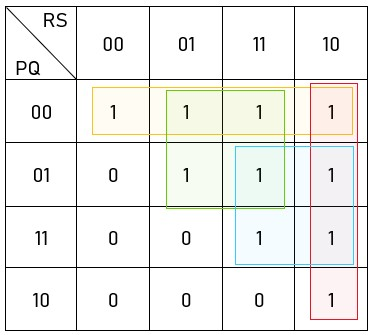
\includegraphics{/mnt/c/Users/manid/FWC/assignment1/KMAP_ASN1}
    \vspace{4pt}
    \caption{Grouped K-map}
    \label{fig:my_label}
\end{table}
Simplified Boolean expression will be:
$$F(P,Q,R,S) = P'Q' + P'S + RS' + QR$$

\section{Verification \& Conclusion}
The simplified Boolean expression can be implemented using 
\\
\\
\vspace{10pt}
\begin{tabular}{|c|}
    \hline

wget https://raw.githubusercontent.com/parusamanideep\\/FWC/tree/main/Assignment1/src/main.cpp

     \\ \hline
\end{tabular} \\
P, Q, R, S are given as inputs to 2, 3, 4, 5 pins respectively from the 5V and GND lines.
\\
\\
The given Boolean expression is simplified and verified for functionality.




\end{document}